

%----------------------------------------------------------------------------------------
%	PACKAGES AND OTHER DOCUMENT CONFIGURATIONS
%----------------------------------------------------------------------------------------

\documentclass[12pt]{article}

\usepackage{polski}
\usepackage[polish]{babel}
\usepackage[utf8]{inputenc}
\usepackage{datetime} 
\usepackage{graphicx}
\usepackage{tikz}
\usepackage{amsmath}
\usepackage{epstopdf}
\usepackage{multirow}
\usepackage{tabularx}
%\usepackage[colorlinks=true]{hyperref}
%\usepackage[all]{hypcap}
%\usepackage{showframe} 
\usepackage{geometry}
 \geometry{
 a4paper, 
 left=20mm,
 right=20mm,
 top=20mm,
 bottom=20mm,
 }
 
%----------------------------------------------------------------------------------------
 
%----------------------------------------------------------------------------------------
% DATES
%----------------------------------------------------------------------------------------

\renewcommand{\dateseparator}{.}
\newdate{exercise_date}{01}{04}{2014}

%----------------------------------------------------------------------------------------

%----------------------------------------------------------------------------------------
% TIKZ PACKAGES
%----------------------------------------------------------------------------------------

\usetikzlibrary{arrows}

%----------------------------------------------------------------------------------------

\begin{document}
 
\begin{titlepage}

\newcommand{\HRule}{\rule{\linewidth}{0.5mm}}
% Defines a new command for the horizontal lines, change thickness here

\center
% Center everything on the page
 
%----------------------------------------------------------------------------------------
%	LOGO SECTION
%----------------------------------------------------------------------------------------


\includegraphics[width=6cm]{../res/img/logo.png}\\[1cm]
% Include a department/university logo - this will require the graphicx package
 
%----------------------------------------------------------------------------------------
 
%----------------------------------------------------------------------------------------
%	HEADING SECTIONS
%----------------------------------------------------------------------------------------

\textsc{\LARGE Akademia Górniczo-Hutnicza \\[0.2cm]
im. Stanisława Staszica w Krakowie}\\[1.5cm]
% Name of your university/college

\textsc{\Large Podstawy Automatyki}\\[0.5cm]
% Major heading such as course name

%----------------------------------------------------------------------------------------
%	TITLE SECTION
%----------------------------------------------------------------------------------------

\HRule \\[0.5cm]
{ \huge \bfseries Dyskretne układy regulacji \\[0.3cm] oraz \\[0.5cm] Analiza
serwomechanizmu \\[0.2cm] przekaźnikowego z wykorzystaniem płaszczyzny
fazowej}\\[0.3cm]
% Title of your document
\HRule \\[1.5cm]
 
%----------------------------------------------------------------------------------------
%	AUTHOR SECTION
%----------------------------------------------------------------------------------------

% \begin{minipage}{0.4\textwidth}
% \begin{flushleft} \large
% \emph{Author:}\\
% Konrad \textsc{Adasiewcz} % Your name
% \end{flushleft}
% \end{minipage}
% ~
% \begin{minipage}{0.4\textwidth}
% \begin{flushright} \large
% \emph{Supervisor:} \\
% dr inż. Paweł \textsc{Rotter} % Supervisor's Name
% \end{flushright}
% \end{minipage}\\[4cm]

% If you don't want a supervisor, uncomment the two lines below and remove the section above
\flushright
\Large \emph{Autorzy:}\\
Konrad \textsc{Adasiewcz}\\[0.1cm] % Your name
Michał \textsc{Maciejewski}\\[3cm] % Your name

%----------------------------------------------------------------------------------------
%	DATE SECTION
%----------------------------------------------------------------------------------------
Data wykonania ćwiczenia: \\
{\large \displaydate{exercise_date}}\\[1cm]


\vfill % Fill the rest of the page with whitespace

\end{titlepage} 

\section{Wstęp}

\subsection{Cel ćwiczenia} 

Celem ćwiczenia jest zapoznanie się z przykładami identyfikacji parametrów modelu rzeczywistego obiektu 
regulacji. Obiekt rzeczywisty jest obiektem nieskończenie wymiarowym, natomiast dla celów sterowania 
zostanie opisany modelami transmitancyjnymi niższych rzędów. 
%następującej postaci:

% \begin{equation*}
% 	\begin{array}{l l}
% 		G_1(s)= & \dfrac{ke^{-s\tau_1}}{sT_o+1} \\[0.5cm]
% 		G_2(s)= & \dfrac{ke^{-s\tau_2}}{(sT_1+1)(sT_2+1)} \\[0.5cm]
% 		G_3(s)= & \dfrac{k}{(sT+1)^n}
% 	\end{array}
% \end{equation*}

\subsection{Przygotowanie punktów pomiarowych do analizy}

Otrzymane dane pomiarowe są obarczone dużymi zakłóceniami, co uniemożliwia
wyznaczenie dyskretnej pochodnej próbek i znalezienie punktu przegięcia metodami
bardziej dokładnymi niż odczucie mierzącego. W celu ich filtracji zastosowany
został dolnoprzepustowy cyfrowy filtr sinc z oknem Blackman'a o częstotliwości
odcięcia $f_c=0.01$ częstotliwości próbkowania.

\begin{figure}[!htp]
	\begin{center}
		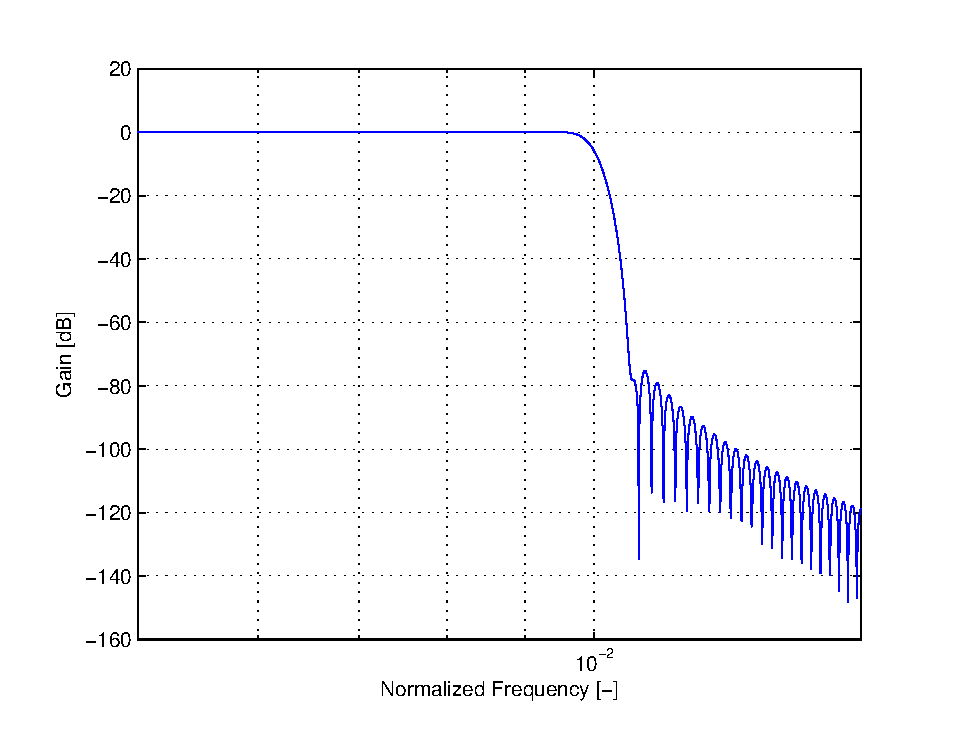
\includegraphics[width=13cm]{../res/img/filresp.eps}
	\end{center} 
	\caption{Charakterystyka częstotliwościowa filtru}
\end{figure}

\newpage

\begin{figure}[!htp]
	\begin{center}
		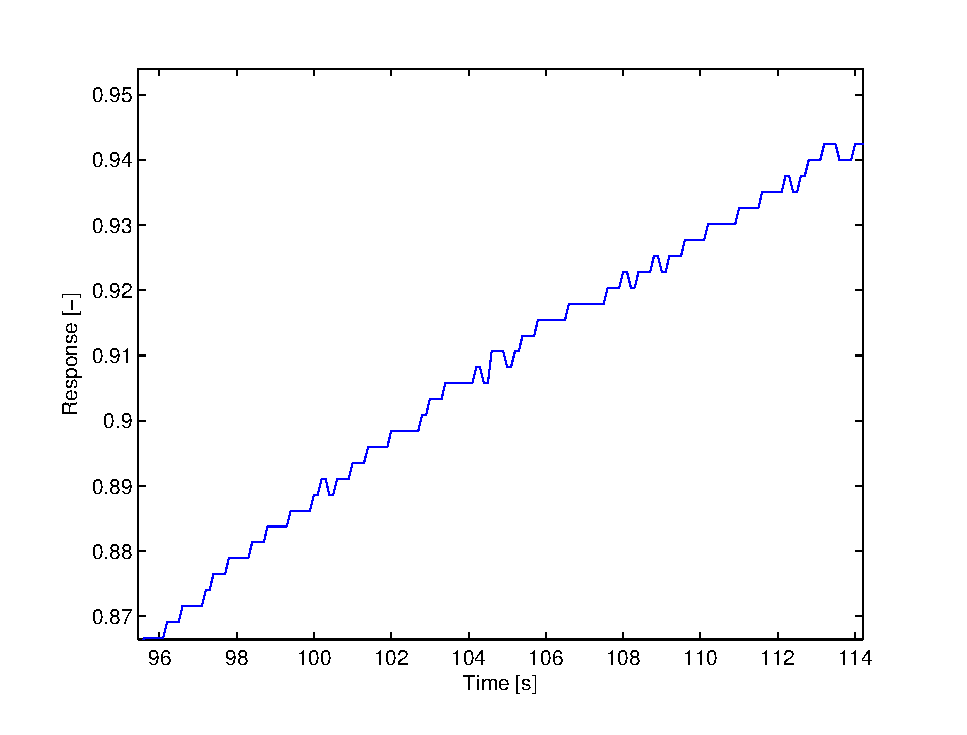
\includegraphics[width=13cm]{../res/img/szum.eps}
	\end{center}
	\caption{Zaszumione próbki odpowiedzi}
\end{figure}

\begin{figure}[!htp]
	\begin{center}
		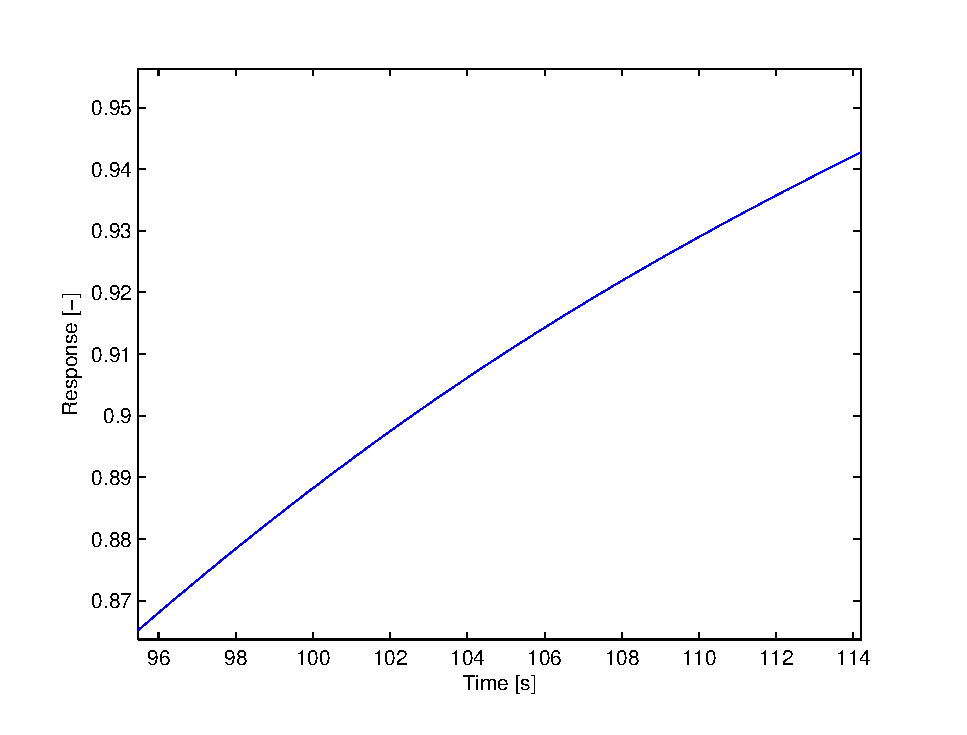
\includegraphics[width=13cm]{../res/img/szumless.eps}
	\end{center} 
	\caption{Przefiltrowane próbki odpowiedzi}
\end{figure}

\newpage

\subsection{Odpowiedź badanego obiektu i jej charakterystyczne parametry}

Poniżej zamieszczony jest czasowy przebieg odpowiedzi badanego obiektu na skok
jednostkowy, wstawioną w punkcie przegięcia przebiegu styczną oraz zaznaczonymi
charakterystycznymi w czasie punktami.

Czasy wystąpienia poszczególnych punktów zaznaczonych na wykresie to:

\begin{equation} 
\begin{array}{r c l}
	t_A&=&21.6[s] \\
	t_{PP}&=&39.9[s] \\
	t_B&=&91.2[s]
\end{array}
\label{equ:params}
\end{equation}

Dodatkowo wartość odpowiedzi w stanie ustalonym $h_{\infty}=1.0712[-]$.

\begin{figure}[!htb]
	\begin{center}
		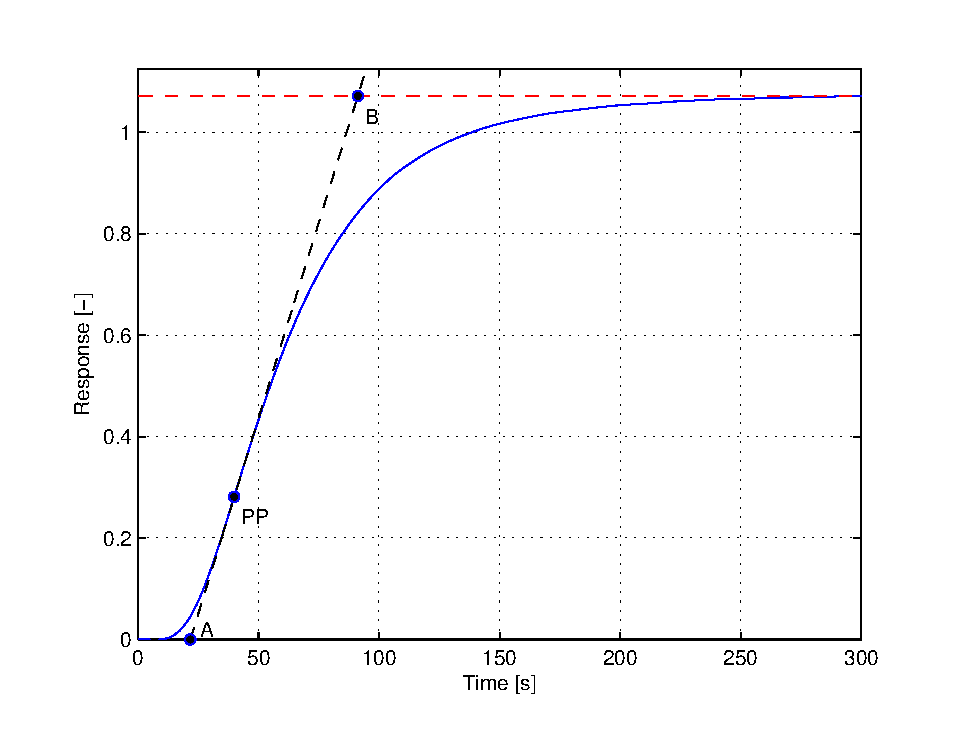
\includegraphics[width=13cm]{../res/img/resppom.eps}
	\end{center} 
	\caption{Odpowiedź badanego obiektu na skok jednostkowy i charakterystyczne
	punkty}
\end{figure}

\newpage

\section{Aproksymacja modelami niskich rzędów}

Ponieważ ustalenie dokładnego modelu badanych w rzeczywistości obietków jest
trudne, a często wręcz niemożliwe, w praktyce inżynierskiej często posługuje się
aproksymacjami przy pomocy uproszczonych modeli niskich rzędów, które posiadają
niewiele parametrów co za tym idzie jesteśmy w stanie je wyznaczyć. Wszystkie
wyznaczone parametry zostaną najpierw przybliżone różnymi metodami graficznymi,
następnie przy pomocy pakietu \textsc{Matlab} zostanie przeszukane ich
bezpośrednie sąsiedztwo metodą \textit{Brute Force} w poszukiwaniu najlepszych
parametrów, z kryterium minimalizacji błędu średniokwadratowego.

Dla każdego z analizowanych modeli stałym i wyznaczonym dokładnie parametrem
jest wzmocnienie $k$, które wynosi:

\begin{equation*}
	k=\frac{h_{\infty}}{1}=1.0712[-]
\end{equation*}
\subsection{Model Kupfmuellera I rzędu z opóźnieniem}

Model Kupfmuellera I rzędu z opóźnieniem jest najprostszym ideowo modelem którym
jesteśmy w stanie z dość przyzwoitą dokładnością przybliżać wiele rodzajów
obiektów rzeczywistych. Transmitancja tego modelu to:

\begin{equation}
	G(s)=\dfrac{ke^{-s\tau}}{sT+1}
	\label{equ:trankup1}
\end{equation}

Mamy więc do wyznaczenia tylko dwa parametry, w dodatku zmiana pojedynczego z
nich oddziałuje na kształt odpowiedzi w przewidywalny sposób, więc ich
wyznaczenie metodami empirycznymi jest proste. Standardowo przyjmuje się
zastępcze parametry następująco:

\begin{equation*}
\begin{array}{r c l}
	\tau&=&t_A=21.6[s] \\
	T&=&t_B-t_{PP}=51.3[s] 
\end{array}
\end{equation*}

Metodą \textit{Brute Force} dochodzimy do optymalnych parametrów:

\begin{equation}
\begin{array}{r c l}
	\tau&=&25.7[s] \\
	T&=&43.6[s] 
\end{array}
\label{equ:paramkup1}
\end{equation}

\begin{figure}[!htp]
	\begin{center}
		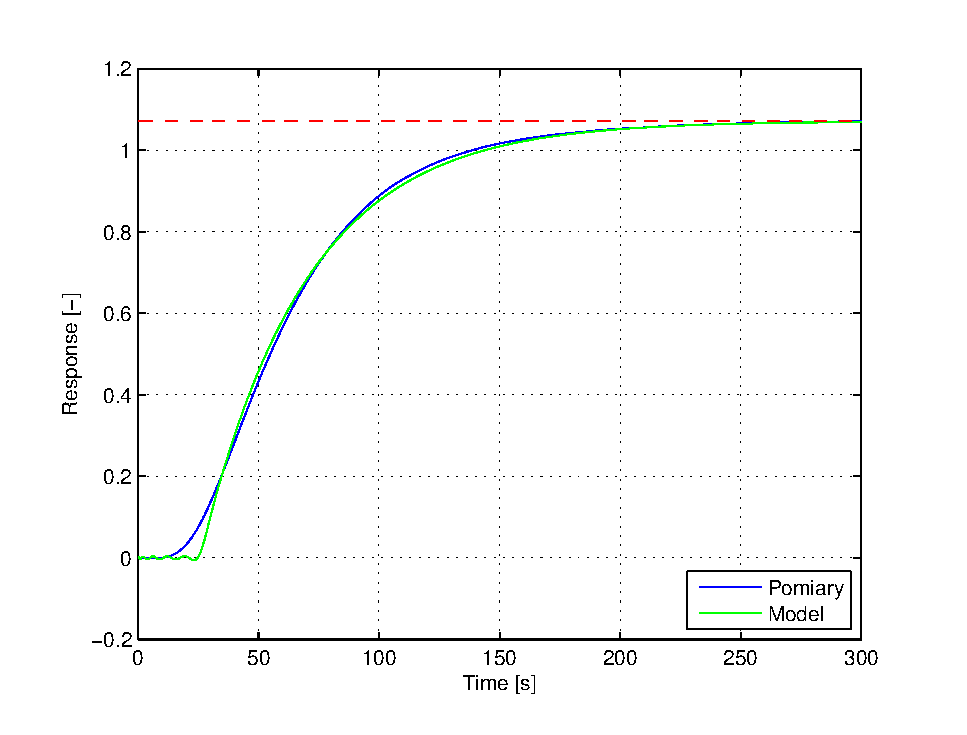
\includegraphics[width=13cm]{../res/img/step11.eps}
	\end{center} 
	\caption{Odpowiedź modelu Kupfmuellera I rzędu z opóźnieniem na tle punktów
	pomiarowych ($\tau=25.7[s]$, $T=43.6[s]$)}
\end{figure}

\begin{figure}[!htp]
	\begin{center}
		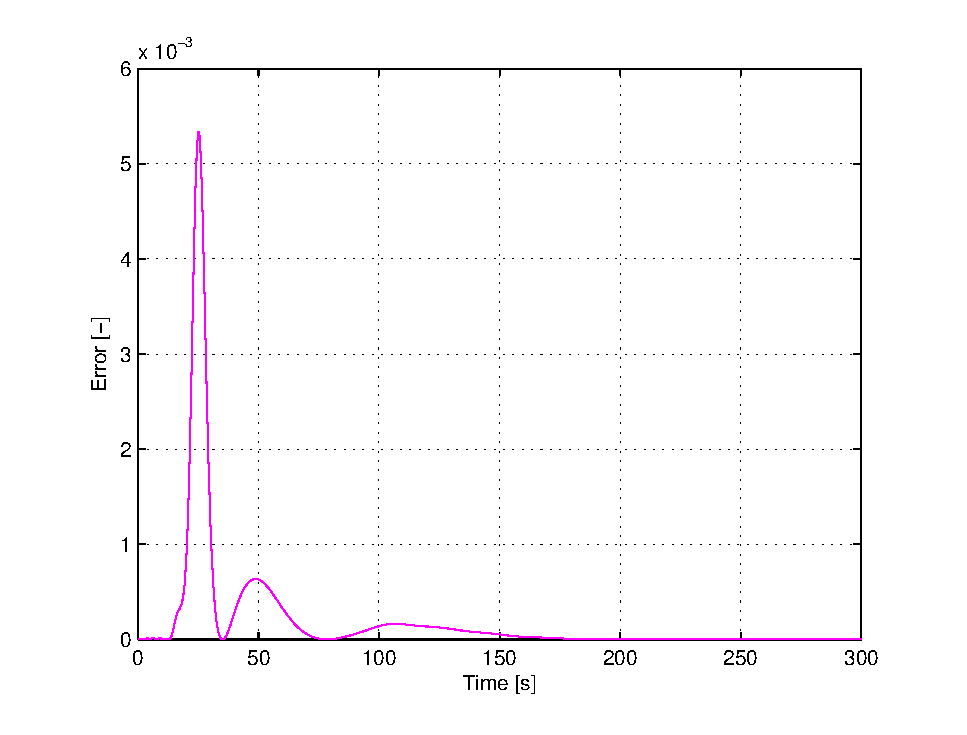
\includegraphics[width=13cm]{../res/img/err11.eps}
	\end{center} 
	\caption{Przebieg błędu w czasie ($\tau=25.7[s]$, $T=43.6[s]$). Całka z błędu
	$\varepsilon=0.05838$}
\end{figure}


\newpage

\subsection{Model Kupfmuellera II rzędu z opóźnieniem}

Transmitancja operatorowa tego modelu wynosi:

\begin{equation}
	G(s)=\frac{ke^{-s\tau}}{(T_1s+1)(T_2s+1)}
	\label{equ:trankup2}
\end{equation}

Kładąc czasy $T_n$ oraz $T_s$ następująco: 

\begin{equation*}
\begin{array}{r c l}
	T_n&=&t_B-t_A=69.6[s] \\
	T_s&=&t_B-t_{PP}=51.3[s] 
\end{array}
\end{equation*}

Przybliżone parametry zastępcze $T_1$ oraz $T_2$ obliczamy z zależności\footnote{
http://www.kssiz.freehost.pl/TSiS\%201\%20-\%20Ch-ki\%20czasowe.pdf}:

\begin{equation*}
	\begin{cases}
		T_1^2+2T_nT_1-T_nT_s=0 \\
		T_2=T_s-T_1
	\end{cases}
\end{equation*}

Dla odpowiedzi badanego obiektu wynoszą one:

\begin{equation*}
	\begin{array}{r c l}
		T_1&=&22.13[s] \\
		T_2&=&29.17[s] 
	\end{array}
\end{equation*}

Parametry optymalne wyznaczone metodą \textit{Brute Force} mają wartości:

\begin{equation*}
	\begin{array}{r c l}
		T_1&=&22.83[s] \\
		T_2&=&29.17[s] \\
		\tau&=&15.13[s]
	\end{array}
\end{equation*}

\newpage

\begin{figure}[!htp]
	\begin{center}
		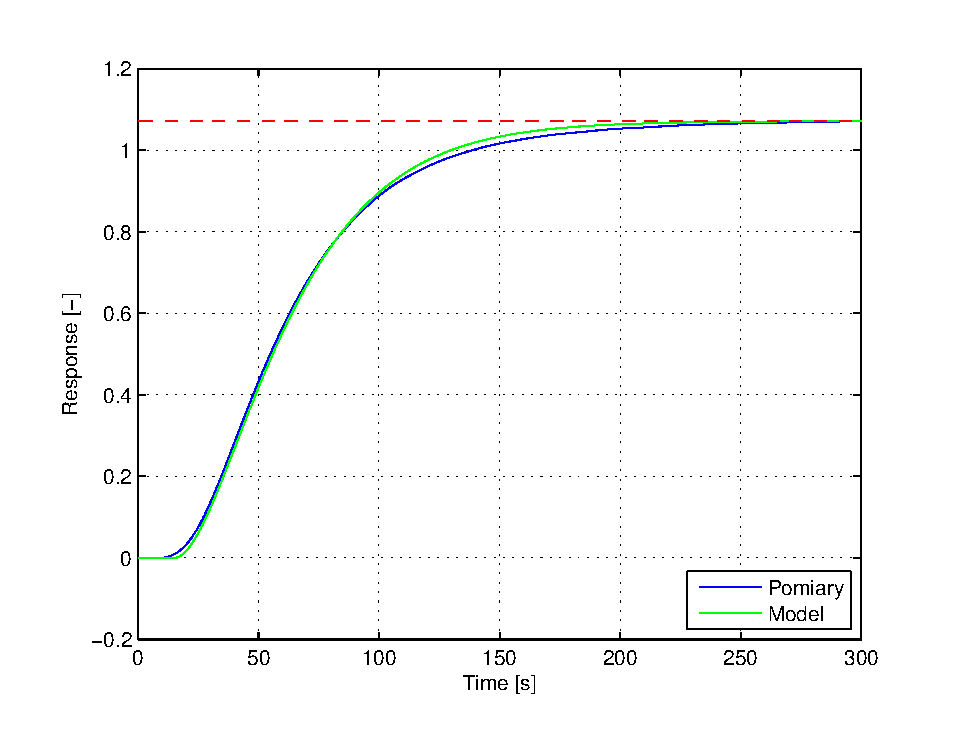
\includegraphics[width=13cm]{../res/img/step21.eps}
	\end{center} 
	\caption{Odpowiedź modelu Kupfmuellera II rzędu z opóźnieniem na tle punktów
	pomiarowych ($\tau=15.13[s]$, $T_1=22.83[s]$, $T_2=29.17[s]$)}
\end{figure}

\begin{figure}[!htp]
	\begin{center}
		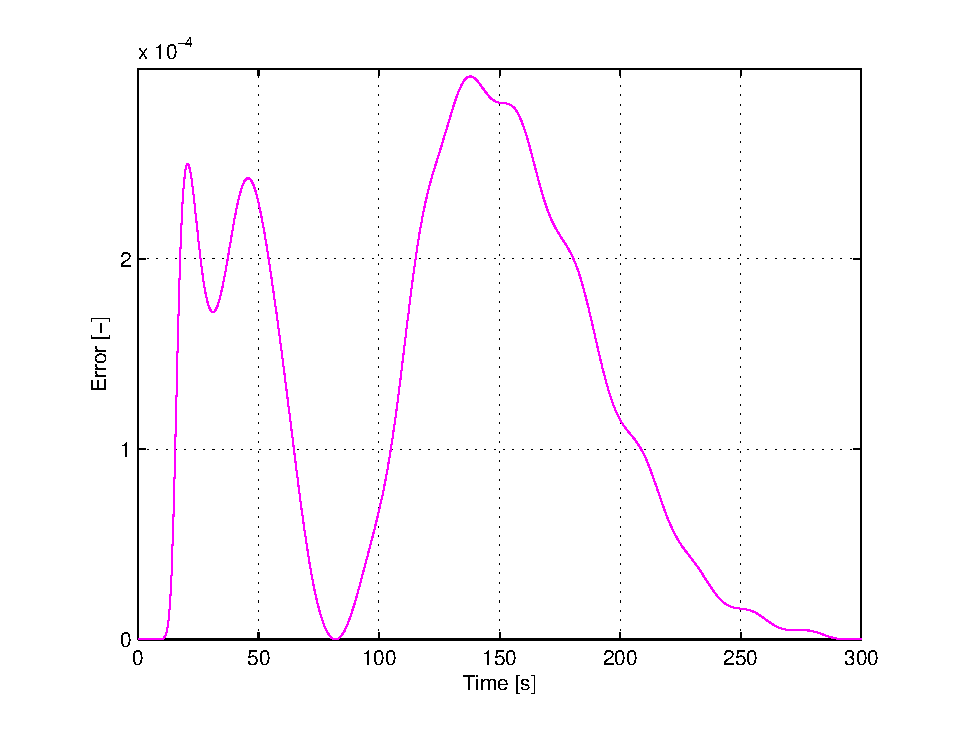
\includegraphics[width=13cm]{../res/img/err21.eps}
	\end{center} 
	\caption{Przebieg błędu w czasie ($\tau=15.13[s]$, $T_1=22.83[s]$,
	$T_2=29.17[s]$).
	Całka z błędu $\varepsilon=0.03602$}
\end{figure}

\newpage

\subsection{Model Strejca}

Transmitancja operatorowa tego modelu wynosi:

\begin{equation}
	G(s)=\frac{k}{(sT+1)^n}
	\label{equ:transtrejc}
\end{equation}

W przypadku tego modelu najprościej dobrać parametry wyjściowe do metody
empirycznie, ponieważ parametr $n$ jest naturalny, więc
zbiór jego rozsądnych wartości do sprawdzenia będzie skończony.
Metodą prób i błędów otrzymałem wyjściowe wartości parametrów $n$ i $T$. Jak
poprzednio metoda \textit{Brute Force} nie zawodzi i dostajemy
następujące wartości parametrów dla których błąd jest minimalny:

\begin{equation*}
	\begin{array}{r c l}
		n&=&3 \\
		T&=&22.06[s]
	\end{array}
\end{equation*}

\newpage

\begin{figure}[!htp]
	\begin{center}
		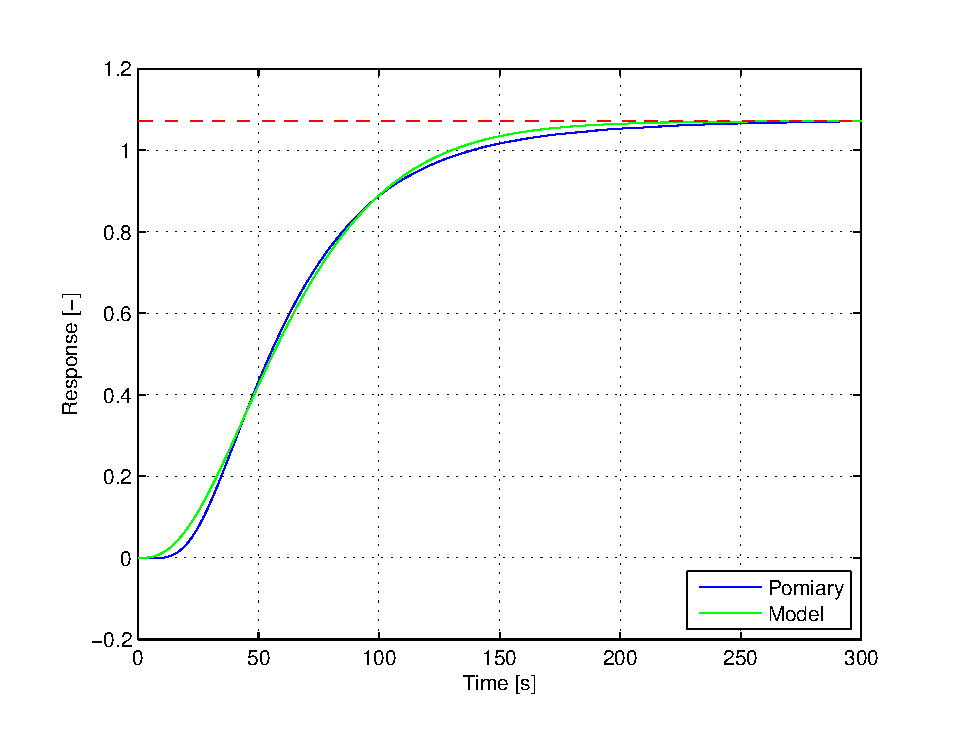
\includegraphics[width=13cm]{../res/img/step31.eps}
	\end{center} 
	\caption{Odpowiedź modelu Strejca na tle punktów
	pomiarowych ($n=3$, $T=22.06[s]$)}
\end{figure}

\begin{figure}[!htp]
	\begin{center}
		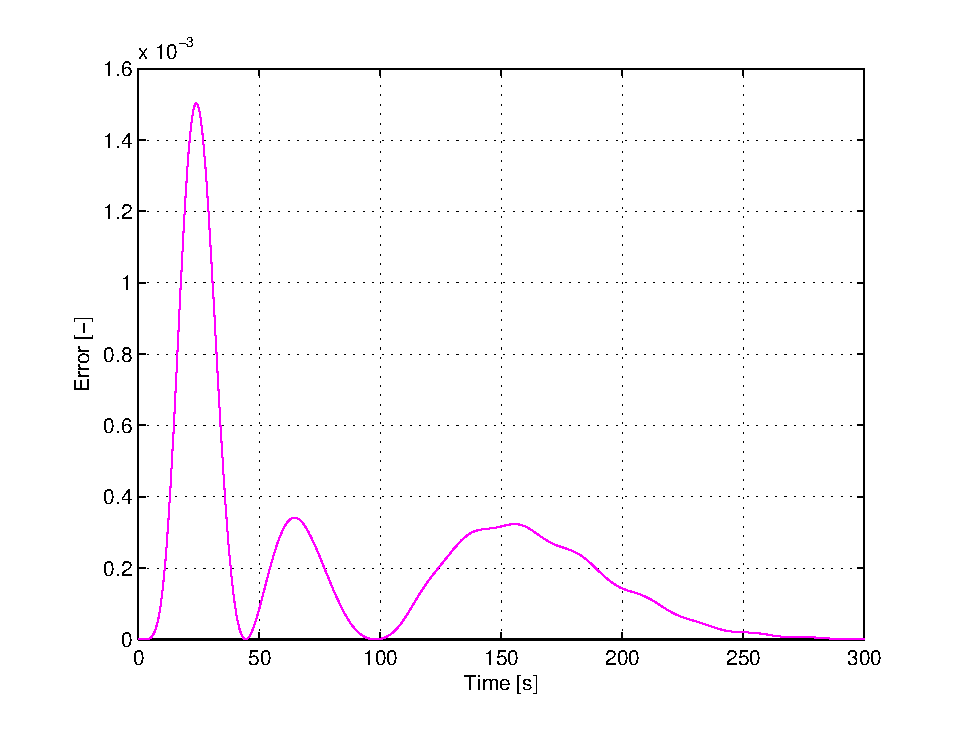
\includegraphics[width=13cm]{../res/img/err31.eps}
	\end{center} 
	\caption{Przebieg błędu w czasie ($n=3$, $T=22.06[s]$). Całka z błędu
	$\varepsilon=0.0608$}
\end{figure}


\newpage

\section{Wnioski i spostrzeżenia}

Otrzymane dane pomiarowe były obarczone znacznymi zakłóceniami wysokiej
częstotliwości, co uniemożliwiało przeprowadzenie analizy kształtu odpowiedzi
metodami bardziej złożonymi niż typowo graficzne. W wyniku filtracji cyfrowej
możliwe było wyznaczenie punktu przegięcia oraz kąta nachylenia krzywej
metodami obliczeniowymi.

Warto wspomnieć również, iż modele z opóźnieniem są
aproksymowane, ponieważ pakiet \textsc{Matlab} jest w stanie przetwarzać
transmitancje jedynie w postaci skończonych ułamków wymiernych, w której to
postaci nie jesteśmy w stanie przedstawić modeli z opóźnieniem, ponieważ
występuje w nich funkcja eksponencjalna.

Modelem, którego odpowiedź najbardziej przypominała odpowiedź badanego
obiektu był model Kupfmuellera II rzędu z opóźnieniem, co nie jest zadziwiające,
ponieważ jest on modelem najbardziej swobodnym z badanych(kształt odpowiedzi
zależał aż od trzech zmiennych).

Warto zauważyć, że pomimo iż model Strejca choć okazał się być najgorszym
przybliżeniem badanego obiektu, jest bardzo wygodny w analizie, ponieważ jego
transmitancja wyrażona jest skończonym ułamkiem wymiernym. Istotną cechą tego
modelu jest również to, iż przestrzeń możliwych do wybrania parametrów dla tego
modelu jest najwęższa, ponieważ jeden z parametrów wyrażony jest liczbą
naturalną, co powoduje iż jest on często wykorzystywany do automatycznej
identyfikacji obiektów.
\end{document}